\documentclass{article}
\usepackage{color}
\usepackage[usenames,dvipsnames]{xcolor}
\usepackage{listings}	
\usepackage{enumerate}
\usepackage{layouts}
\usepackage{times}
\usepackage[numbers]{natbib}
\usepackage{notoccite}
\usepackage{todonotes}
\usepackage{alltt}
\usepackage{url}
\usepackage{amsmath}
\usepackage{amsfonts}
\usepackage{amsthm}
\usepackage{xspace}
\usepackage{tikz}
\usepackage[dvipsnames]{xcolor}
\usepackage{subcaption}

\usepackage{fancyvrb}

\theoremstyle{definition}
\newtheorem{definition}{Definition}[section]
\newcommand{\triple}[1]{\ensuremath{\langle #1 \rangle}}
\newcommand{\pair}[1]{\ensuremath{\left(#1\right)}}
\newcommand{\graph}[1]{\ensuremath{\mathcal{#1}}}
\newcommand{\graphset}[1]{\ensuremath{\mathfrak{#1}}}

% redefine \VerbatimInput
\RecustomVerbatimCommand{\VerbatimInput}{VerbatimInput}%
{fontsize=\footnotesize,
   %
  frame=lines,  % top and bottom rule only
  framesep=2em, % separation between frame and text
  rulecolor=\color{Gray},
      %
  label=\fbox{\color{Black}proB encoding},
  labelposition=topline,
        %
% commandchars=\|\(\), % escape character and argument delimiters for
                              % commands within the verbatim
% commentchar=*        % comment character
}

\author{Authors}
\title{Note on KR and Graph Mining}
\begin{document}
\maketitle

\section{Introduction}

Machine learning techniques often contain a process of learning certain patterns from a set of graphs.
This problem, which exists in many forms, is called the \emph{Graph Mining} problem.
\todo{Wat verantwoording en extra info vragen aan Sergey over waarom dit probleem interessant is. Ook is dit 'structured' graph mining, er bestaan andere vormen geloof ik, hoe bespreken we die?}

%\subsection{Problem definition}
\begin{definition}
\label{def:GM1}
Given a pair $\pair{E_{+},E_{-}}$ consisting of a set of \emph{positive} and \emph{negative} examples of \emph{labeled graphs}, respectively,
\emph{Graph mining} is the problem of finding one \emph{connected labeled graph} $P$, called a \emph{pattern},
that is \emph{homomorphic} with at least $N_{+}$ positive, while homomorphic with at most $N_{-}$ negative examples.
\end{definition}

\begin{definition}
A graph $\graph{G} = \triple{V,E,L}$, where $V$ is the set of vertices, $E$ the set of edges and $L$ the labeling function, is \emph{connected} iff for each pair of vertices $v$ and $v'$, there exists an edge $\pair{v,v'} \in E$ or there exists a sequence $v \ldots v_{1} \ldots v_{n} \ldots v'$ such that there exist edges $\pair{v,v_{1}}$, $\pair{v_{i},v_{i+1}}$ and $\pair{v_{n},v'} \in E$.
\end{definition}


\begin{definition}
A graph homomorphism $f$ between two labeled graphs $\graph{G} = (V,E,L)$ and $\graph{G'} = (V',E',L')$, where $V$ is the set of vertices, $E$ the set of edges and $L$ the labeling function, is a mapping $V \rightarrow V'$ from vertices of $\graph{G}$ to vertices of $\graph{G'}$ s.t. 
\begin{itemize}
\item $\forall u,v \in V, \pair{u,v} \in E \implies \pair{f(u),f(v)} \in E'$ (the mapping preserves edges), and 
\item $\forall v \in V : L(v) = L(f(v))$ (the mapping respects labelings).
\end{itemize}
If there exists such a graph homomorphism between graphs $\graph{G}$ and $\graph{G'}$ we say $\graph{G}$ is \emph{homomorphic} with $\graph{G'}$.
\end{definition}

\begin{figure}[h]
    \centering
\begin{subfigure}[b]{0.3\textwidth}
    \centering
    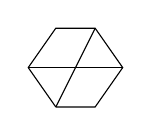
\begin{tikzpicture}[scale=.5]
	    \draw (1,1) -- (2,1) -- (2.7,2) -- (2,3) -- (1,3) -- (0.3,2) -- (1,1);
	    \draw (1,1) -- (2,3);
	    \draw (2.7,2) -- (0.3,2);
    \end{tikzpicture}
    \caption{Positive Example\label{fig:pos}}
\end{subfigure}
~
\begin{subfigure}[b]{0.3\textwidth}
    \centering
    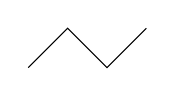
\begin{tikzpicture}[scale=.5]
        \coordinate (1) at (0,0);
        \coordinate (2) at (1,1);
        \coordinate (3) at (2,0);
        \coordinate (4) at (3,1);
        \draw (1) -- (2) -- (3) -- (4);
    \end{tikzpicture}
    \caption{Negative Example\label{fig:neg}}
\end{subfigure}
~
\begin{subfigure}[b]{0.3\textwidth}
    {
    \setcounter{subfigure}{0}
    \renewcommand\thesubfigure{\Roman{subfigure}}
    \centering
	\begin{subfigure}[b]{0.45\textwidth}
	    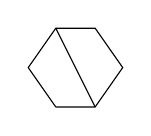
\begin{tikzpicture}[scale=.5]
	        \draw (1,1) -- (2,1) -- (2.7,2) -- (2,3) -- (1,3) -- (0.3,2) -- (1,1);
	        \draw (2,1) -- (1,3);
    	\end{tikzpicture}
    	\caption{Valid\label{fig:correctcandidate}}
	\end{subfigure}
    ~
    \begin{subfigure}[b]{0.45\textwidth}
        \begin{tikzpicture}[scale=.5]
            \draw (1,2) -- (2,3) -- (3,3);
        \end{tikzpicture}
        \caption{Invalid\label{fig:incorrectcandidate}}
    \end{subfigure}
    }
    \caption{Pattern Candidates\label{fig:candidates}}
\end{subfigure}
\caption{Example 1:\label{fig:ex1}}
\end{figure}

%    \begin{tikzpicture}[scale=.5]
%        \coordinate (1) at (0,0);
%        \coordinate (2) at (1,1);
%        \coordinate (3) at (2,0);
%        \coordinate (4) at (3,1);
%        \draw (1) --
%              (2) --
%              (3) --
%              (4);
%    \end{tikzpicture}, ...

Take, for example, the problem set shown in Figure~\ref{fig:ex1}.
There is one positive example (Fig~\ref{fig:pos}), and one negative example (Fig~\ref{fig:neg})
We assume all nodes have the same label.
Figure \ref{fig:candidates} shows a few possible patterns.
Requiring at least one homomorphism with a positive example, and allowing no homomorphisms with negative examples (i.e. problem parameters $N_{+}=1$ and $N_{-}=0$), only Figure \ref{fig:correctcandidate} represents a valid pattern.
It is clear that there exists a mapping from each node from the valid pattern to a node of the positive example, while no such mapping exists for the negative example.
Looking at Figure \ref{fig:correctcandidate}, this graph clearly maps to both the positive as well as the negative example. Therefore, it is not a pattern.

\subsection{Multiple patterns}
To extend on this task, we can look for multiple patterns, instead of just one.
In this case, one can impose restrictions on the different patterns that are found.
For example, it stands to reason that one wants only \emph{canonical} solutions, meaning that no two patterns found are \emph{isomorphic}.

\begin{definition}
\label{def:isomorphism}
A graph isomorphism $f$ between two labeled graph $\graph{G} = \triple{V,E,L}$ and $\graph{G'} = \triple{V',E',L'}$ is a \emph{one-to-one} mapping $V \rightarrow V'$ 
such that $f$ represents a homomorphism from $\graph{G}$ to $\graph{G'}$,
and its inverse $f^{-1}$ represents a homomorphism from $\graph{G'}$ to $\graph{G}$.
If there exists such a graph isomorphism between $\graph{G}$ and $\graph{G'}$ we say $\graph{G}$ and $\graph{G'}$ are \emph{isomorphic}.
\end{definition}


\begin{definition}
\label{def:canonicalForm}
Let $\graphset{G}$ be a set of graphs, closed under isomorphism.
A function $c$ for which $\forall \graph{G,H} \in \graphset{G} : \graph{G} \simeq \graph{H} \iff c(\graph{G}) = c(\graph{H})$ and $\forall \graph{G} \in \graphset{G} : \graph{G} \simeq c(\graph{G})$ hold, is called a \emph{canonization}.
The graph $c(\graph{G})$ is called the \emph{canonical form} w.r.t $c$, and is denoted by $\mathit{canon}(\graph{G})$.
\end{definition}

\begin{figure}[h]
\centering
\begin{subfigure}[b]{0.45\textwidth}
    \centering
    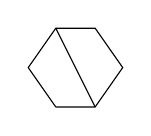
\begin{tikzpicture}[scale=.5]
	    \draw (1,1) -- (2,1) -- (2.7,2) -- (2,3) -- (1,3) -- (0.3,2) -- (1,1);
	    \draw (2,1) -- (1,3);
    \end{tikzpicture}
    \caption{First candidate pattern\label{fig:iso1}}
\end{subfigure}
~
\begin{subfigure}[b]{0.45\textwidth}
    \centering
    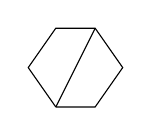
\begin{tikzpicture}[scale=.5]
	    \draw (1,1) -- (2,1) -- (2.7,2) -- (2,3) -- (1,3) -- (0.3,2) -- (1,1);
	    \draw (1,1) -- (2,3);
    \end{tikzpicture}
    \caption{Second candidate pattern\label{fig:iso2}}
\end{subfigure}
\caption{Possible patterns\label{fig:isomorphism}}
\end{figure}

Given the graph mining problem as specified in Figure~\ref{fig:ex1}, we have already established that Figure~\ref{fig:iso1} is a valid pattern.
When we try to mine a second pattern, we might suggest a pattern as shown in Figure~\ref{fig:iso2}.
A quick check, however, will show that there is a one-to-one mapping $f$ such that both $f$ as well as its inverse $f^{-1}$ preserve edges.
As a result, the first candidate pattern and the second are isomorphic.
By Definition~\ref{def:canonicalForm} only one of these two patterns can be the canonical form, and therefore only one of these two candidate patterns should be accepted as a valid pattern.

\subsection{Rewording}

An attempt to model the Graph Mining problem in both IDP as well as ProB makes it clear
that neither language allows us to express the problem to its full extent.
We now try to link the shortcomings of each language to the expressiveness of the underlying logic on which they are built.

First we introduce a new definition of the graph mining problem, equivalent to \textbf{Def.}~\ref{def:GM1}.
We'll assume a sufficiently large supply of vertices, and represent example graphs directly as a triple $\triple{Edge, Label, Class}$, consisting of an edge relation and a labeling function over the vertices, as well as a classification (positive/negative).

\begin{definition} \textbf{Graph Mining (redefined)}
\label{def:gm2}
Given a set of vertices $V$ and a set $\graphset{G}$ of $\triple{E, L, C}$ triples,
where $E$ and $L$ represent the edge relation and labeling function over the supply of vertices respectively,
%which consist of an edge relation, 
we look for a (set $P$ of) \todo{cleanly extend this definition to multiple graphs, or separate the single and multiple pattern case again} graph(s) represented by tuple(s) $\pair{E_{p}, L_{p}}$ such that
for at least $N_{+}$ of the triples $\triple{ E, L, C}$ with $C=Pos$, and for at most $N_{-}$ of such triples with $C=Neg$, there exists a function $f$ s.t. $\forall u,v \in V, \pair{u,v} \in E_{p} \implies \pair{f(u),f(v)} \in E$ and $\forall v \in V : L_{p}(v) = L(f(v))$.

\todo{draft: possible different wording}
\begin{itemize}
\item $\#\Big\lbrace \triple{E,L,Pos} \; | \; \triple{E,L,Pos} \in \graphset{G} \; \wedge \; \big(\exists f : \forall v \in V : L_{p}(v) = L(f(v)) \; \wedge \; \forall x,y \in V : E_{p}(x,y) \implies E(f(x),f(y))\big)\Big\rbrace \geq N_{+}$

\item $\#\Big\lbrace \triple{E,L,Neg} \; | \; \triple{E,L,Neg} \in \graphset{G} \; \wedge \; \big(\exists f : \forall v \in V : L_{p}(v) = L(f(v)) \; \wedge \; \forall x,y \in V : E_{p}(x,y) \implies E(f(x),f(y))\big)\Big\rbrace \leq N_{-}$
\end{itemize}
\end{definition}

This definition shows great \emph{local coherence} with respect to the different graphs: all characteristics of a graph are represented by separate entities or concepts, which are grouped together for each graph $G$ in the triple that describes it.
A natural choice to represent the set of triples would be a (ternary) predicate.
As the domains of this predicate range over predicates and functions, this predicate would be a higher-order predicate.

\todo{Illustrate local coherence with table}
\begin{table}[h]
\centering
\begin{tabular}{l |l l l}
         & E      & L      & C \\
\hline
$\graph{G}_{1}$  & $E_{1}$ & $L_{1}$ & Pos\\
$\graph{G}_{2}$  & $E_{2}$ & $L_{2}$ & Pos\\
  \vdots & \vdots  & \vdots  & \vdots\\
$\graph{G}_{n}$  & $E_{n}$ & $L_{n}$ & Pos\\
\end{tabular}
\caption{Local coherence\label{Fig:LocalCoherence}}
\end{table}



\section{Modellings}
\subsection{IDP}
\subsubsection{Existential Second Order}
The IDP language can expresses problems that consist of a set of symbols, called the vocabulary $V$, and a theory, called $T$, that uses symbols from this vocabulary.
The symbols in the vocabulary can be propositions, but they can also represent predicates and functions.
These last two types of symbols make the vocabulary, in general, \emph{second order}.
The theory $T$ is restricted to a \emph{first order} theory, extended with arithmetic, aggregates, and inductive definitions.
Our inference of choice in the graph mining problem is model expansion; we search for an interpretation $I$ of symbols in the vocabulary $V$ such that this interpretation $I$ satisfies the theory $T$.
This corresponds to the implicit \emph{existential quantification} of all symbols in the vocabulary, both the first order as well as the second order symbols.
In conclusion, we say IDP can express model expansion for \emph{Existential Second Order} problems. 

%problems in which there is an existentially quantified, generally second order, vocabulary of symbols and a first order theory with symbols from that vocabulary.

The restriction to \emph{Existential} Second Order means we cannot express the set of example graphs, as specified in Definition~\ref{def:gm2}, as a higher-order predicate.
One possible solution is to replicate for each graph the different characteristic predicates and functions, as well as the knowledge (theory) about them.
It is clear that this solution is undesirable due to the way it scales and the editing needed with growing problem instances.
It retains the local coherence of graph characteristics when it comes to data representation, but prohibits the abstraction (generalization) of knowledge about these properties, as evidenced by our obligation to duplicate the theory for each graph.

Another solution would be to use a trick where we represent each characteristic property by a single general entity for all graphs that behaves the way it should for a specific graph instance based on an additional argument serving as an identifier for the graph of interest.
It is clear that this trick forces us to give up the local coherence of graph characteristics that was present in \textbf{Def.}~\ref{def:gm2}.

%Nu kunnen we kijken wat deze truuk doet met onze mogelijkheid om de abstraction van de theory uit te drukken. Normaal mwillen we dit zo schrijven. Hoewel we nu de generalisatie kunnen uitdrukken, verplicht de restrictie tot existentieel s..o ons om de homomorphic mapping functies te tot een globale property te promoveren, hoewel we feitelijk niet geinteresseerd zijn in de concrete mappings. om om te gaan met de afhankelijkheid van deze functies op de spec. vb grafen moeten we... die nu erg lijkt op skolemisation. theory

%Using this trick however, does not influence our ability to 
But, can we now express the abstraction (generalization) of knowledge about these properties, such as the positive homomorphic property.
%to separate the constraint describing the positive homomorphic property, and the coint on its number of occurrences.
%This, from a KR point of view, 
%Furthermore, the restriction to ESO requires us 
%As an example, we illustrate this trick by showing on the expression of the positive homomorphic property, where it greatly resembles Skolemization.
As evidenced in \textbf{Def.}~\ref{def:gm2}, normally one would express the positive homomorphic property by quantifying (counting) over all graphs, requiring the existence of a function with the correct properties.
Using this trick, does not influence our ability to express this restriction.

However, the restriction to ESO forbids us to quantify over higher-order entities such as functions outside of the vocabulary.
Thus, we are required to promote the homomorphic mapping functions to a global property, even though we are only interested in the existence of a mapping, and not in a concrete valid mapping itself.
We prevent the same explosion of mapping functions as with the graph characteristics above, using the same trick as above (which in this case corresponds to Skolemization):
We introduce a general function \verb|f| that represents all homomorphisms, and make its dependency on a specific example graph explicit using an additional argument:
\verb|partial f(graph, t_var):node|.
%As it is impossible
%We introduce a general function \verb|f| that represents the homomorphisms, and make its dependency on a specific goal graph explicit using an additional argument:
In Second Order Logic, this dependency would follow directly from the order of the separate quantifications.

We can now use this \verb|f| anywhere we would the regular homomorphic function for a specific graph by fixing the goal graph.
Note that this encoding also requires us to make this function \verb|f| partial, as the Graph Mining problem does not require the solution to be homomorphic with \emph{all} goal graphs.
%\todo{Of course, other (even uglier) schemes exist to encode this. Should we mention this?}

Much in the same way, limiting ourselves to existential second order prohibits us from expressing the constraint negative constraint on homomorphism (No more than $N_{-}$ negative examples are homomorphic) in the same model.
In fact, the negative constraint asserts a property for all candidate homomorphic functions, which would lead to \emph{universal} quantification.
Therefore, our only recourse is to encode its dual positive constraint and require it to fail when queried.

\subsubsection{Inductive Definitions}
Beyond the Existential Second Order restriction, the IDP language is also extended with inductive definitions. These definitions, evaluated under the well-founded semantics, allows the derivation of negative knowledge that otherwise would be underivable.
\reversemarginpar
\todo{A section about inductive definitions, and their use. (Being able to derive negative knowledge)}

\subsection{Eventual encoding}
\begin{alltt}
//Homomorphism/2 is a higher-order predicate:
//Edge1 and Edge2 are predicates themselves.
homomorphism(<Edge1,Label1>, <Edge2,Label2>) 
\(\iff \exists\) f: (\(\forall\) x, y : x \(\neq\) y \(\Rightarrow\) f(x) \(\neq\) f(y)) \(\wedge\)
    (\(\forall\)x, y : Edge1(x, y) \(\implies\) Edge2(f (x), f (y))) \(\wedge\)
    (\(\forall\) x : Label1(x) = Label2(f(x)))
    

\textbraceleft
    reachable(x,y,Edge) \(\leftarrow\) Edge(x,y) \(\lor\) Edge(y,x).
    reachable(x,y,Edge) \(\leftarrow \exists\) : reachable(x,z,Edge) \(\wedge\) reachable(z,y,Edge).
\textbraceright

isomorph(Edge1,Edge2) \(\iff \exists\)f : (\(\forall\) x,y:Edge1(x,y) \(\iff\) Edge2(f(x),f(y))) \(\wedge\)
    (\(\forall\) x : Label1(x) = Label2(f(x))) \(\wedge\)
    (\(\forall\)x,y:x\(\neq\)y\(\implies\)f(x)\(\neq\)f(y)).

//\(\forall\)Pat represents quantification over a predicate Pat/2. 
//A pattern is represented by its Edge relation. 
\(\forall\)P : pattern(P) \(\implies\) #\textbraceleft Pos : positive(Pos) \(\wedge\) homomorphism(P, Pos) \textbraceright \(\geq\) \(N{+}\).
\(\forall\)P : pattern(P) \(\implies\) #\textbraceleft Neg : negative(Neg) \(\wedge\) homomorphism(P, Neg) \textbraceright \(\leq\) \(N_\).
\(\forall\)P,P2 :pattern(P)\(\wedge\)pattern(P2)\(\wedge\)P\(\neq\)P2 \(\iff\) \(\neg\)isomorph(P,P2).

\end{alltt}
\reversemarginpar
\todo{Tekstuele uitleg hierbij}

\subsection{ProB}

\section{Feature Comparison}

\subsection{IDP} 

\textbf{Pro:}
\begin{itemize}
  \item can model inductive definitions
  \item allows core formulation in a high-level language (NP)
  \item handles aggregates
  \item has support for variety of constraints
\end{itemize}
\textbf{Cons:}
\begin{itemize}
  \item cannot handle negative case $\textit{NP}^\textit{NP}$ complexity
  \item cannot model subgraph isomorphism independence
  \item cannot handle dominance, i.e., when one model is preferred over another 
\end{itemize}

\paragraph{ASP}
Mostly the same but in theory can handle $\textit{NP}^\textit{NP}$, in practice however, it would require encoding tricks and unavoidably lead to the same problem as in IDP -- indexing homomorphism enumeration.

\lstset{basicstyle=\footnotesize\ttfamily,breaklines=true}
\begin{lstlisting}[caption=ASP positive matching]
positive_match(G) | not_positive_match(G) :- positive(G).

1 { map(G,X,V) : node(G,V) } 1 :- positive(G), invar(X).

:- positive_match(G), map(G,X,V1), map(G,Y,V2), t_edge(X,Y), 
                  not edge(G,V1,V2), invar(X), invar(Y).

positive_count(N) :- N = #count{G:positive_match(G)}.

:- positive_count(N), N < 2.
\end{lstlisting}

\begin{lstlisting}[caption=ASP negative matching]
%Saturated Representation

%negative constraints to check not matching negative graphs

map(G,X,v1) | map(G,X,v2) | map(G,X,v3) | map(G,X,v4) :- invar(X), negative(G).

map(G,X,V) :- saturated(G), t_node(X), node(G,V).

saturated(G) :- t_edge(X,Y), map(G,X,V1), map(G,Y,V2), not edge(G,V1,V2), negative(G), invar(X), invar(Y).
saturated(G) :- map(G,X,V),  map(G,Y,V), X != Y, invar(X), invar(Y). // we cannot map two different template nodes to the same 

negative_match(G) :- not saturated(G), negative(G).

negative_count(N) :- N = #count{G:negative_match(G)}.

:- negative_count(N), N > 1.

\end{lstlisting}

\begin{lstlisting}[caption=Canonicity template-based check]
iso(X,x1) | iso(X,x2) | iso(X,x3) | iso(X,x4) :- invar(X).

candidate_var(X) :- iso(_,X).

%not iso!
iso_saturated :- invar(X1), invar(X2), iso(X1,V1), iso(X2,V2),     t_edge(V1,V2), not t_edge(X1,X2). 
iso_saturated :- invar(X1), invar(X2), iso(X1,V1), iso(X2,V2), not t_edge(V1,V2),     t_edge(X1,X2).
 
iso(X,V) :- invar(X), t_node(V), iso_saturated.

d1(X) :-     invar(X), not candidate_var(X). 
d2(X) :- not invar(X),     candidate_var(X).

not_equal :- d1(X). % check that in fact candidate is different from the pattern itself
not_equal :- d2(X). % check that in fact candidate is different from the pattern itself

iso_saturated :- not not_equal. % should not be completely equal

min_d1(N) :- N = #min{ X: d1(X) }, not iso_saturated.
min_d2(N) :- N = #min{ X: d2(X) }, not iso_saturated.

iso_saturated :- min_d1(N1), min_d2(N2), N1 > N2.
\end{lstlisting}

\begin{lstlisting}[caption=Auxilary predicates -- probably should be moved to appendix]
%selects subpattern

t_path(X,Y) :- t_edge(X,Y), invar(X), invar(Y).
t_path(X,Y) :- t_edge(X,Z), t_path(Z,Y), invar(X).

:- invar(X), invar(Y), not t_path(X,Y).

0 { invar(X) } 1 :- t_node(X).
% auxilary constraints


edge(G,Y,X) :- edge(G,X,Y).
t_edge(Y,X) :- t_edge(X,Y).
node(G,Y)   :- edge(G,Y,_).
t_node(X)   :- t_edge(X,_).
\end{lstlisting}

\begin{lstlisting}[caption=Canonicity previous solution isomorphism check]
iso(s1,X,x1) | iso(s1,X,x2) :- invar(X).
iso(s2,X,x2) | iso(s2,X,x3) :- invar(X).

candidate_var(G,X) :- iso(G,_,X).

iso_saturated(G) :- invar(X1), invar(X2), iso(G,X1,V1), iso(G,X2,V2),     t_edge(V1,V2), not t_edge(X1,X2). 
iso_saturated(G) :- invar(X1), invar(X2), iso(G,X1,V1), iso(G,X2,V2), not t_edge(V1,V2),     t_edge(X1,X2). 
iso_saturatea(G) :- not equal(G), iso(G,_,_). 

iso(G,X,V) :- invar(X), t_node(V), iso_saturated(G).

:- not iso_saturated(G), iso(G,_,_).

d1(G,X) :-     invar(X), not candidate_var(G,X), iso(G,_,_).
d2(G,X) :- not invar(X),     candidate_var(G,X).

not_equal(G) :- d1(G,X). % check that in fact candidate is different from the pattern itself
not_equal(G) :- d2(G,X). % check that in fact candidate is different from the pattern itself

equal(G) :- not not_equal(G), iso(G,_,_).
\end{lstlisting}


\subsection{proB}
\textbf{Pro:}
\begin{itemize}
  \item can model negative case
  \item can model subgraph isomorphism independence
\end{itemize}
\textbf{Cons:}
\begin{itemize}
  \item cannot handle inductive definitions
  \item cannot handle different types of aggregates (? needs to be checked again)
\end{itemize}

the rest of constraints? 

\section{Code in ProB and IDP}

\VerbatimInput{original_prob_files/PositiveAndNegative.mch}
\pagebreak

\VerbatimInput[label=IDP encoding]{IDPencoding/core_constraints.idp}



\end{document}
